\documentclass[]{book}
\usepackage{lmodern}
\usepackage{amssymb,amsmath}
\usepackage{ifxetex,ifluatex}
\usepackage{fixltx2e} % provides \textsubscript
\ifnum 0\ifxetex 1\fi\ifluatex 1\fi=0 % if pdftex
  \usepackage[T1]{fontenc}
  \usepackage[utf8]{inputenc}
\else % if luatex or xelatex
  \ifxetex
    \usepackage{mathspec}
  \else
    \usepackage{fontspec}
  \fi
  \defaultfontfeatures{Ligatures=TeX,Scale=MatchLowercase}
\fi
% use upquote if available, for straight quotes in verbatim environments
\IfFileExists{upquote.sty}{\usepackage{upquote}}{}
% use microtype if available
\IfFileExists{microtype.sty}{%
\usepackage{microtype}
\UseMicrotypeSet[protrusion]{basicmath} % disable protrusion for tt fonts
}{}
\usepackage[margin=1in]{geometry}
\usepackage{hyperref}
\hypersetup{unicode=true,
            pdftitle={StatPREP: Data-driven statistics},
            pdfauthor={Daniel Kaplan},
            pdfborder={0 0 0},
            breaklinks=true}
\urlstyle{same}  % don't use monospace font for urls
\usepackage{natbib}
\bibliographystyle{apalike}
\usepackage{longtable,booktabs}
\usepackage{graphicx,grffile}
\makeatletter
\def\maxwidth{\ifdim\Gin@nat@width>\linewidth\linewidth\else\Gin@nat@width\fi}
\def\maxheight{\ifdim\Gin@nat@height>\textheight\textheight\else\Gin@nat@height\fi}
\makeatother
% Scale images if necessary, so that they will not overflow the page
% margins by default, and it is still possible to overwrite the defaults
% using explicit options in \includegraphics[width, height, ...]{}
\setkeys{Gin}{width=\maxwidth,height=\maxheight,keepaspectratio}
\IfFileExists{parskip.sty}{%
\usepackage{parskip}
}{% else
\setlength{\parindent}{0pt}
\setlength{\parskip}{6pt plus 2pt minus 1pt}
}
\setlength{\emergencystretch}{3em}  % prevent overfull lines
\providecommand{\tightlist}{%
  \setlength{\itemsep}{0pt}\setlength{\parskip}{0pt}}
\setcounter{secnumdepth}{5}
% Redefines (sub)paragraphs to behave more like sections
\ifx\paragraph\undefined\else
\let\oldparagraph\paragraph
\renewcommand{\paragraph}[1]{\oldparagraph{#1}\mbox{}}
\fi
\ifx\subparagraph\undefined\else
\let\oldsubparagraph\subparagraph
\renewcommand{\subparagraph}[1]{\oldsubparagraph{#1}\mbox{}}
\fi

%%% Use protect on footnotes to avoid problems with footnotes in titles
\let\rmarkdownfootnote\footnote%
\def\footnote{\protect\rmarkdownfootnote}

%%% Change title format to be more compact
\usepackage{titling}

% Create subtitle command for use in maketitle
\newcommand{\subtitle}[1]{
  \posttitle{
    \begin{center}\large#1\end{center}
    }
}

\setlength{\droptitle}{-2em}
  \title{StatPREP: Data-driven statistics}
  \pretitle{\vspace{\droptitle}\centering\huge}
  \posttitle{\par}
  \author{Daniel Kaplan}
  \preauthor{\centering\large\emph}
  \postauthor{\par}
  \predate{\centering\large\emph}
  \postdate{\par}
  \date{2018-03-02}

\usepackage{booktabs}
\usepackage{amsthm}
\makeatletter
\def\thm@space@setup{%
  \thm@preskip=8pt plus 2pt minus 4pt
  \thm@postskip=\thm@preskip
}
\makeatother

\usepackage{amsthm}
\newtheorem{theorem}{Theorem}[chapter]
\newtheorem{lemma}{Lemma}[chapter]
\theoremstyle{definition}
\newtheorem{definition}{Definition}[chapter]
\newtheorem{corollary}{Corollary}[chapter]
\newtheorem{proposition}{Proposition}[chapter]
\theoremstyle{definition}
\newtheorem{example}{Example}[chapter]
\theoremstyle{definition}
\newtheorem{exercise}{Exercise}[chapter]
\theoremstyle{remark}
\newtheorem*{remark}{Remark}
\newtheorem*{solution}{Solution}
\begin{document}
\maketitle

{
\setcounter{tocdepth}{1}
\tableofcontents
}
\chapter{Teaching Data-driven Statistics}\label{intro}

Description, prediction, decision

Large and growing student interest in computer science and statistics.
That growing interest is not simply a matter of new subjects receiving
attention or of transient employment opportunities. The interest
reflects systemic changes in the technical infrastructure of life and
work in the US and the world due to the emergence of ubiquitous
computing. Among other things, computing has led to an explosion in the
availability of data and to the ability to explore systems at a greater
level of complexity and a finer level of detail. Since computers always
work with a mathematical representation of the world, the ability to
construct and interpret such representations (aka ``modeling'') is now a
core part of research, commercial, industrial, medical, social, and
government activities. Mathematical skills, particularly in applied math
and statistics, are essential here.

\begin{enumerate}
\def\labelenumi{\arabic{enumi}.}
\tightlist
\item
  Wrangling
\item
  Visualization
\item
  Statistical description
\item
  Prediction
\end{enumerate}

\section{Pocket guide to StatPREP
commands}\label{pocket-guide-to-statprep-commands}

See \texttt{Essential\_statprep\_command.key}. Maybe put a copy of it
here, or a full-page version.

\chapter{Data and Presentations}\label{data-and-presentations}

Here is a very general, dictionary definition of ``data''

\begin{quote}
factual information (as measurements or statistics) used as a basis for
reasoning, discussion, or calculation --
\href{https://www.merriam-webster.com/dictionary/data}{Merriam-Webster
dictionary}
\end{quote}

Let's re-organize this definition into three components: raw facts;
calculation; reasoning and discussion. These three components translate
into three broad classes of data:

\begin{enumerate}
\def\labelenumi{\arabic{enumi}.}
\tightlist
\item
  \textbf{Non-tabular data} which can be any record, be it in the form
  of notes from interviews, photographs, sound and signal recordings,
  readings from lab instruments, documents, medical records, etc. These
  are the ``facts'' in the dictionary definition.
\item
  \textbf{Tabular data}, a spreadsheet-like organization, which is by
  far the most widely used for statistical calculation.
\item
  \textbf{Data presentations}, that is, data formatted in a way to be
  more-or-less directly accessible to human perception, discussion, and
  reasoning. One of the most useful forms of data presentation is
  graphics, but there are others.
\end{enumerate}

We'll be mainly concerned with the calculations by which tabular data is
transformed into presentations. The tabular format for data provides a
standard that makes it straightforward to perform many of the
calculations, allows different software tools to interoperate, and
provides the mean to combine data from different sources in creative and
flexible ways.

\section{Non-tabular data}\label{non-tabular-data}

As an example of non-tabular data, consider the records from one of the
earliest statistical projects, Francis Galton's investigation in the
1880s of the heritability of biological traits. Records of Galton's
collection of data on the heights of adult children and their parents
are contained in Galton's notebook, a portion of which is displayed in
Figure 1.

\begin{figure}
\centering
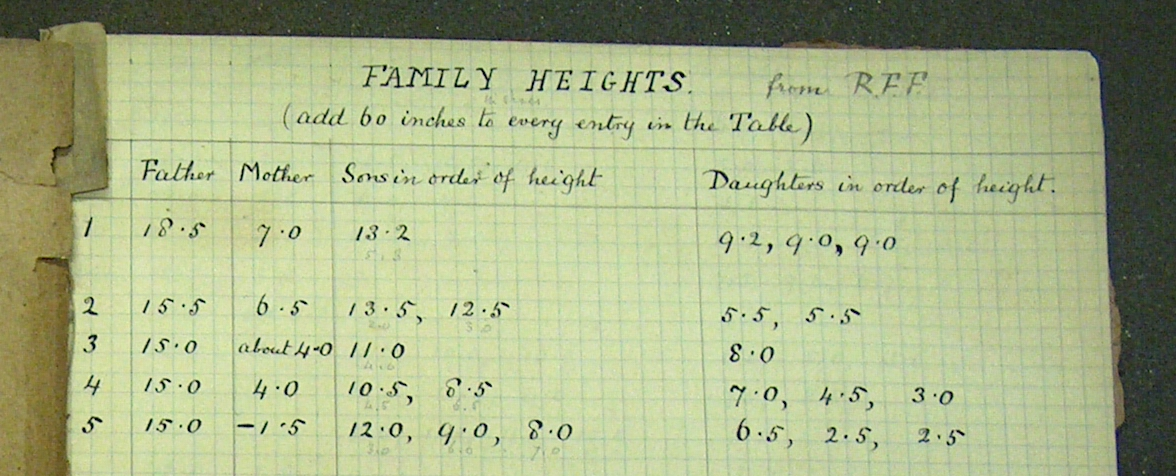
\includegraphics{images/galton-notebook.jpg}
\caption{}
\end{figure}

Figure 1: \emph{Part of a page from Francis Galton's notebook.}

You can imagine how Galton might have collected these data, going from
house to house in London, tacking a yardstick to a wall, and having the
various members of the family stand in front of the ruler to measure
their heights. A yardstick isn't a suitable length to measure height
from the floor to the head, so perhaps Galton positioned the yardstick
at a height of 5 feet above the floor and recorded the number of extra
inches above that. So recording a daughter with a height of 9.2 means
that her actual height was 5 ft 9.2 inches, or 69.2 inches.

Galton's notebook is neatly organized, but it's raw data, not in the
kind of tabular form used in statistical calculations.

\section{Tabular data}\label{tabular-data}

Tabular data is organized as a rectangular array. There are two
coordinates to a rectangle, and similarly there are two coordinates to
tabular data:

\begin{enumerate}
\def\labelenumi{\arabic{enumi}.}
\tightlist
\item
  Rows, also called ``cases'' or ``units of observation.''
\item
  Columns, also called ``variables''
\end{enumerate}

Here's one possible organization of the height measurements in Galton's
notebook rendered into a tabular form:

\begin{verbatim}
## PhantomJS not found. You can install it with webshot::install_phantomjs(). If it is installed, please make sure the phantomjs executable can be found via the PATH variable.
\end{verbatim}

\hypertarget{htmlwidget-0041afc6eb1e2aad9d36}{}

Figure 2: \emph{Galton's notebook observations translated to a tabular
form.}

\section{Data presentations}\label{data-presentations}

You can page through the Galton data table but it is very hard to draw
conclusions from the table itself. \emph{Data presentations} show data
in a manner better suited for interpretation by people. The proper
design of the presentation depends on its \emph{purpose}: what aspect of
the data you wish to emphasize. There can be very different
presentations of the same data for different purposes.

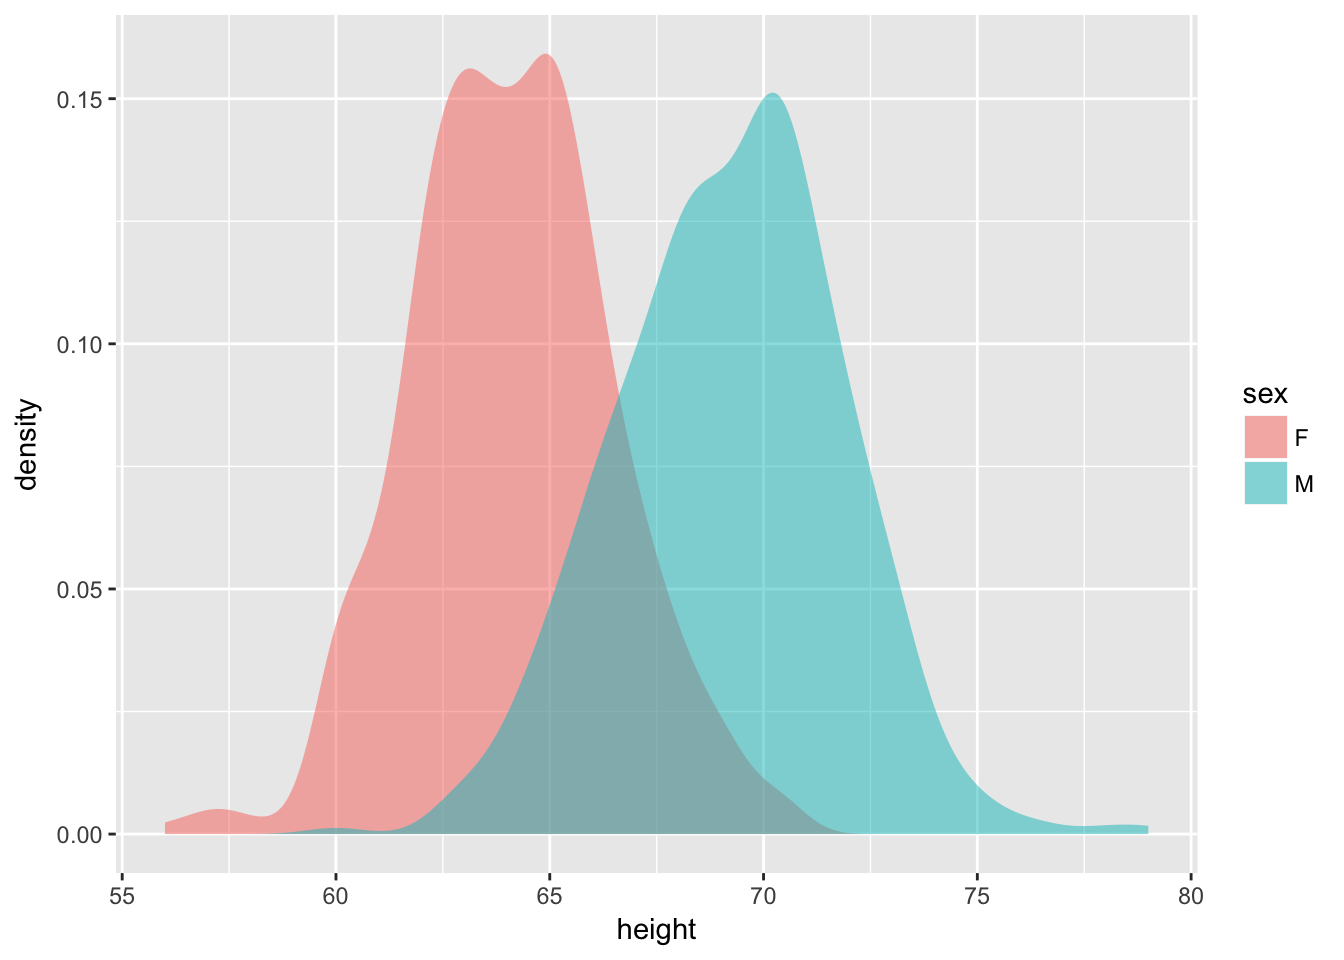
\includegraphics{statprep-notes_files/figure-latex/unnamed-chunk-2-1.pdf}

Figure 3: \emph{A graphical presentation of Galton's data for the
purpose of comparing heights by sex.}

Presentations often are numerical in form, such as this report of the
means and standard deviations of the heights of the girls and boys in
Galton's data.

\begin{verbatim}
##   sex        m        s
## 1   F 64.11016 2.370320
## 2   M 69.22882 2.631594
\end{verbatim}

Or, consider this rather more technical presentation on the difference
in mean heights between the sexes:

\begin{verbatim}
##    estimate statistic       p.value  conf.low conf.high
## 1 -5.118656 -30.66182 1.042115e-141 -5.446293 -4.791018
\end{verbatim}

Much of what we teach in intro stats is about familiarizing students
with a variety of forms of data presentations and how to draw
conclusions from them.

\chapter{Data Frames}\label{data-frames}

something here

\section{Rows and columns}\label{rows-and-columns}

Data tables are organized into rows and columns.

\begin{itemize}
\tightlist
\item
  Each row is a \emph{unit of observation}.
\item
  Each column is a \emph{variable}.
\end{itemize}

\subsection{Unit of observation}\label{unit-of-observation}

The \emph{unit of observation} is the kind of thing each row corresponds
to in the real world. In Figure 2, the unit of observation is a child.
Galton recorded heights of 898 children in his notebook so there are 898
rows in the data table.

In a properly arranged data table, every row is about the same sort of
observational unit. If you have different types of observational units,
they should be in different tables. For instance, you might have a table
giving the address of each family. That should not be intermixed with
the table where the unit of observation is a child. Instead, it would be
in a separate table where the unit of observaton is a family.

\subsection{Variables}\label{variables}

Each column of a data table is a \emph{variable}. The individual entries
in the column are \emph{values} of the variable. The word ``variable''
reflects that the values vary from row-to-row.

In the Galton table, there are six different variables:

\begin{enumerate}
\def\labelenumi{\arabic{enumi}.}
\tightlist
\item
  An ID for the family.
\item
  The family's father's height. (inches)
\item
  The family's mother's height. (inches)
\item
  The sex of the child.
\item
  The child's height. (inches)
\item
  The number of children in the family.
\end{enumerate}

In properly arranged tabular data, the value for any particular variable
is the \emph{same kind of thing} for every observational unit. For
instance, the \texttt{father} variable is the height of the father in
inches. Values of the \texttt{sex} variable are always ``F'' or ``M''.

\section{Kinds of values}\label{kinds-of-values}

Data tables are composed of two main types of variables:

\begin{enumerate}
\def\labelenumi{\arabic{enumi}.}
\tightlist
\item
  \textbf{Quantitative}: a number.
\item
  \textbf{Categorical}: a label, typically written using characters.
\end{enumerate}

In the Galton data table, the \texttt{sex} variable is categorical and
consists of the labels \texttt{"F"} and \texttt{"M"}. The other
variables are quantitative. But note that the \texttt{family} variable,
although expressed as numbers, is actually a categorical variable: all
that matters about the values in \texttt{family} is that they are
distinct. The order is of no particular meaning; we can't say that
family 4 is in between families 2 and 5.

Quantitative variables typically represent some real-world quantity such
as height, age, blood pressure, etc. Such real-world quantities often
have \emph{units}, e.g.~inches, years, millimeters of mercury (mmHg).

In a properly organized data table, the units of the quantitative
variable are \emph{not} part of the value; they are implicit. A good
reason for this is that in properly organized data, the a variable's
unit should be the same in every row. This is part of what it means that
all the values are \emph{the same kind of thing}.

For a categorical variable, the set of possible values of the variables
are called the \emph{levels} of the variable. In the Galton \texttt{sex}
variable, the set consists of \texttt{"F"} and \texttt{"M"}.

\subsection{Missing data}\label{missing-data}

In both quantitative and categorical values are sometimes
\emph{missing}. Historically, such missingness was often denoted with a
special numerical value such as \texttt{-999} or with a special level
such as \texttt{"missing"}. This is a poor practice, since it's easy to
mistakenly treat those values as if they were non-missing. Instead, a
special token is used to indicate missing data: \texttt{NA}.

\section{The codebook}\label{the-codebook}

How are you to know what are the physical units of a quantitative
variable or the legitimate levels of a categorical variable? This
information is contained in a \emph{codebook} associated with the data
table. Codebook can take the form of an actual book, a text file, a
spreadsheet, a PDF document, etc.

Many of the data tables we will be working with have codebooks available
through the R \texttt{help()} system. For instance, the following
command chunk will display the codebook for the \texttt{Galton} data
table:

\section{Tables and files}\label{tables-and-files}

Data tables are typically stored as computer files. There are many
formats for such files in use. One popular file format is called
\emph{CSV} (comma-separated values). The particular file format does not
really matter, so long as you can find the appropriate software to read
the file. Similarly, the physical location of the file does not really
matter, so long as you have access to it.

\subsection{Loading data}\label{loading-data}

When using statistical software, data tables are ``read in'' to the
software. This is often called \emph{loading} the data table. The R
statistical software has a standard representation of a data table,
called a ``data frame.'' There are several widely used implementations
of data frames and so you may see referenced to \texttt{data.frame},
\texttt{tibble}, etc.

In general, a first step in using data is to load the data from a file
into a data frame. Almost always, the data frame is given a name by
which the table can be referred.

The following command chunk has two commands. The first reads in a small
data table from a file on the internet, creating a data frame given the
name \texttt{Baseball}. The second causes the data frame to be printed.

\begin{verbatim}
## # A tibble: 14 x 3
##    Team         Wins BattingAvg
##    <chr>       <int>      <dbl>
##  1 New York       97      0.285
##  2 Toronto        87      0.284
##  3 Baltimore      70      0.277
##  4 Boston         86      0.269
##  5 Tampa Bay      61      0.255
##  6 Cleveland      78      0.280
##  7 Detroit        95      0.274
##  8 Chicago        90      0.280
##  9 Kansas City    62      0.271
## 10 Minnesota      96      0.287
## 11 Los Angeles    89      0.274
## 12 Texas          80      0.278
## 13 Seattle        78      0.272
## 14 Oakland        93      0.260
\end{verbatim}

\subsection{R-package data}\label{r-package-data}

Many of the data tables we will use in these notes have already been
loaded into R by instructing R to use a \emph{library} or \emph{package}
containing the data. This is the case with the \texttt{Galton} example,
which comes from the \texttt{mosaicData} package.

For the present, you don't need to be concerned with how to load
R-package data. It will be done for you. But do remember that somewhere
there is a computer file containing the data and that it is being loaded
in to R with software appropriate for that format of file.

\section{Textbook data}\label{textbook-data}

Recall the distinction between tabular data and a \emph{presentation}
constructed from the data. Textbooks are oriented to the human reader
and, naturally, they tend to use forms indended for the human reader.
Thus, much of the ``data'' in textbooks is in the form of presentations
such as the cross-tabulation in Figure 1.

\begin{figure}
\centering
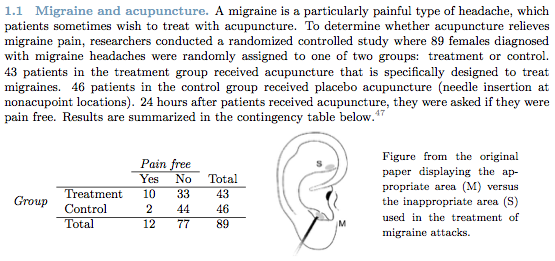
\includegraphics{images/migrane-isrs1.png}
\caption{}
\end{figure}

Figure 1: \emph{A data presentation from the open source textbook
``Intro Stat with Simulation and Randomization''
\href{https://www.openintro.org/stat/textbook.php?stat_book=isrs}{ISRS}.}

A stickler might argue that the table in Figure 1 can be construed as a
data table, but for our purpose here, let's take a pragmatic approach to
defining what constitutes the sorts of data used in data science. In
particular, these notes will focus on data that contain many rows and
are available in machine-readable form. Or, stated another way, we'll
work with data \emph{before} they have been aggregated into the sort of
presentation seen in Figure 1.

It's easy to imagine what the disaggregated data table that underlies
this presentation might look like: perhaps this one where the unit of
observation is a person:

\begin{longtable}[]{@{}lllll@{}}
\toprule
patient & accupuncture & pain & date & technician\tabularnewline
\midrule
\endhead
A2322 & control & yes & 2014-03-15 & Audrey\tabularnewline
A2397 & treatment & yes & 2014-03-17 & Audrey\tabularnewline
A3213 & treatment & no & 2014-03-17 & Bill\tabularnewline
B8732 & treatment & no & 2014-03-18 & Audrey\tabularnewline
C6920 & control & yes & 2014-03-18 & Bill\tabularnewline
\(\vdots\) & \(\vdots\) & \(\vdots\) & \(\vdots\) &
\(\vdots\)\tabularnewline
\bottomrule
\end{longtable}

Figure 2: \emph{What the underlying data from Figure 1 might have looked
like, presented as a data table.}

By learning the tools to work with data tables, you can easily create
presentations like the cross-tabulation in Figure 1. But you also have
the ability to explore other possible explanations for the variation in
pain, such as the effectiveness of the technician or the day of the
week.

\section{Example}\label{example}

Figure 3 shows a style of presentation common in intro stats textbooks.

\begin{figure}
\centering
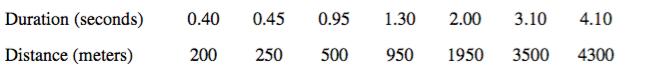
\includegraphics{images/Data-honeybees.png}
\caption{}
\end{figure}

\begin{figure}
\centering
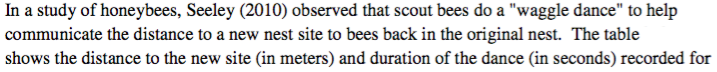
\includegraphics{images/Data-honeybees-1.png}
\caption{}
\end{figure}

Figure 3: \emph{A textbook presentation of data (Source: 2016 GAISE
College Report)}

The data are almost in tabular form. Does it matter that the variables
are arranged as rows rather than columns? Not in any mathematical sense,
but it is a violation of the standard format for data, which means that
the data will be (slightly) more difficult to work with: you'll have to
transform them to the standard before performing calculations.

The textbook provides a brief description of the data, including an
explanation of the meaning of the variables and their units, and an
indication of the source. Since data tables are usually stored as a
computer file, such descriptive information is stored in an auxilliary
file called a ``codebook.''

Note that the variable names --- \texttt{Duration\ (seconds)} and
\texttt{Distance\ (meters)} --- include the units. This is appropriate
in a data presentation. But the data table from which this presentation
originates should not include the units; that information can be placed
in the codebook.

Figure 4 shows two imagined data-table forms for the honeybee data. The
left form has included the units --- seconds and meters. In the left
table, the two variables are actually categorical, not numeric. Look
closely at the printed table. Under the variable name, it includes a
brief description of the type of variable. \texttt{chr} stands for
``character'', which is to say that the variables in the left table are
being stored as character strings. The table on the right properly
presents the values as numeric. (The notation \texttt{dbl} refers to a
particular internal format for the numbers, a
``double-precision-floating point number''. You will also see, from time
to time, \texttt{int}, which indicates that the number is stored in
computer integer format. In your calculations, you don't need to worry
about which type of storage format is used for numerical data.)

Improper form

Proper form

\begin{tabular}{l|l}
\hline
duration & distance\\
\hline
0.40 sec & 200 m\\
\hline
0.45 sec & 250 m\\
\hline
0.95 sec & 500 m\\
\hline
1.30 sec & 950 m\\
\hline
\end{tabular}

~

\begin{tabular}{r|r}
\hline
duration & distance\\
\hline
0.40 & 200\\
\hline
0.45 & 250\\
\hline
0.95 & 500\\
\hline
1.30 & 950\\
\hline
\end{tabular}

\begin{tabular}{cc}
Improper form & Proper form\\

\begin{tabular}{l|l}
\hline
duration & distance\\
\hline
0.40 sec & 200 m\\
\hline
0.45 sec & 250 m\\
\hline
0.95 sec & 500 m\\
\hline
1.30 sec & 950 m\\
\hline
\end{tabular}

 & 
\begin{tabular}{r|r}
\hline
duration & distance\\
\hline
0.40 & 200\\
\hline
0.45 & 250\\
\hline
0.95 & 500\\
\hline
1.30 & 950\\
\hline
\end{tabular}

\\
\end{tabular}

Figure 4: \emph{Two possible ways of arranging the honeybee data in a
data table. The left one is awkward: the variables are categorical even
though they represent physical quantities. The right table properly has
quantitative variables: their values are numbers. The physical meaning
for the number is described in the codebook, which here takes the form
of descriptive text in the book.}

\chapter{Organizing stats}\label{organizing-stats}

Much emphasis in stats courses is given to the arithmetic involved in
calculating statistics such as the mean and standard deviation. This
might be a valid way to introduce concepts, but in data science the
computation of the statistic itself is a trivial (but essential!) part
of the overall work. The difficult part is keeping track of the results
so that they can be presented and so that they can play a role in
additional calculations.

For instance, presenting the mean with its confidence interval involves
computing these statistics: the mean, the standard deviation, \(n\).
Glueing them together into the confidence interval requires more
operations: addition, subtraction, division, square roots, and (for very
small \(n\)) looking up a value from the t-distribution.

Such a complicated sequence of operations makes a good example for an
introductory programming course. Even the programming involved in
storing a confidence interval (a pair of numbers) exercises substantial
programming skills.

Keeping the whole process in mind, even when using familiar tools such
as paper and pencil, imposes a substantial cognitive load and distracts
from the main objective: drawing meaningful conclusions from data. Our
objective here is to streamline the process so that we can think about
how to use statistics rather than how to calculate statistics.

\bibliography{book.bib}


\end{document}
